    \documentclass[11pt,letterpaper]{article}
    \usepackage[utf8]{inputenc}
    \usepackage{amsmath}
    \usepackage{amsfonts}
    \usepackage{amssymb}
    \usepackage{geometry}
    \usepackage{hyperref}
    \usepackage{xcolor}
    \usepackage{booktabs}
    
    % Brand Typography / Color configuration
    \definecolor{mpdark}{HTML}{0F172A}
    \definecolor{mpblue}{HTML}{3B82F6}
    \definecolor{mpgreen}{HTML}{10B981}
    \definecolor{mpred}{HTML}{EF4444}
    \definecolor{mpblack}{HTML}{000000}
    
    \usepackage{float} 
    \usepackage{graphicx}
    \graphicspath{{visual-assets/}} % Looks in the relative images folder
    
    % Clean, modern margins
    \geometry{margin=1in}
    
    \hypersetup{
        colorlinks=true,
        linkcolor=mpblue,
        urlcolor=mpblue
    }
    
    \title{\textbf{\color{mpdark}Money Plot Labs Technical Whitepaper \\ The Pure Math of Financial Freedom}}
    \author{\textbf{Harrison Hsueh} \\ \textit{Founder, Money Plot Labs}}
    \date{May 2026}
    
    \begin{document}
    
    \maketitle
    
    \begin{abstract}
    This whitepaper derives the explicit, closed-form analytical solution for a fixed-horizon retirement timeline. By presenting a simple linear model first, we establish a transparent baseline using middle-school algebra. We then expand this model into exponential growth curves by mapping the exact continuous boundaries between an asset accumulation phase and an annuity-due depletion phase. This isolates the exact number of required working years ($w$) as a function of savings rate, spending targets, initial capital, investment growth, and desired legacy floors.
    \end{abstract}
    
    \section{Introduction \& Variables}
    Standard personal finance paradigms rely on fragile rules of thumb. To achieve absolute mathematical certainty, we model an individual's financial lifecycle across a strictly bounded timeline from a starting age ($T_{\text{start}}$) to a maximum life expectancy ($T_{\text{end}}$). We define the total planning horizon as:
    \begin{equation}
    H = T_{\text{end}} - T_{\text{start}}
    \end{equation}
    
    Within this horizon $H$, an individual works for $w$ consecutive years and spends the remaining $f$ years in full retirement, such that:
    \begin{equation}
    H = w + f
    \end{equation}
    
    \subsection{Parameter Definitions}
    \begin{itemize}
        \item $A_0$: Initial Net Worth / Starting Balance (\$)
        \item $c$: Annual Cash Savings Flow during working years (\$)
        \item $b$: Annual Retirement Budget Consumption (\$)
        \item $L$: Desired Capital Legacy Floor / Inheritance Remaining at Death (\$)
        \item $r$: Real Growth Rate adjusted for inflation
        \item $w$: Accumulation Phase duration (Working Years)
        \item $f$: Depletion Phase duration (Retirement Years)
    \end{itemize}
    
    ---
    
    \section{The Linear Baseline Case ($r = 0\%$)}
    % =========================================================================
    % SECTION: PLOT 1 (LINEAR INTERSECTION BASELINE)
    % =========================================================================
    \begin{figure}[H]
    \centering
    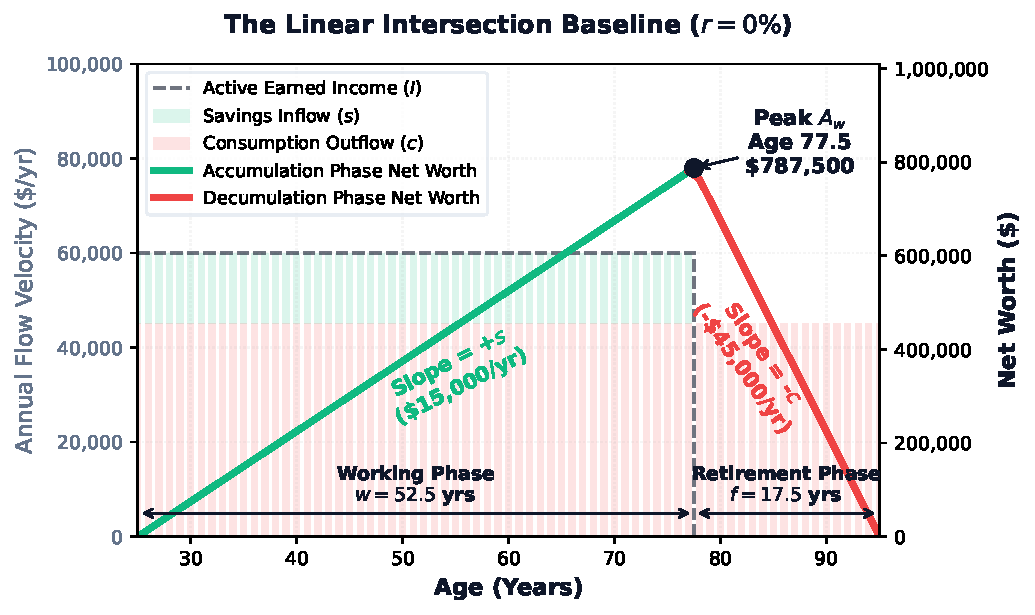
\includegraphics[width=12cm, height=6cm]{linear_plot.pdf}
    \caption{The straight-line boundary crossover mapping where $r =0\%$. Assets accumulate smoothly via \textcolor{mpgreen}{labor} and deplete symmetrically via \textcolor{mpred}{consumption} until hitting the legacy boundary.}
    \label{fig:linear_plot}
    \end{figure}
    Before introducing the compounding curves of financial markets, we establish an intuitive baseline by assuming real asset growth perfectly tracks inflation ($r = 0\%$). In this environment, wealth accumulates and depletes along perfectly straight lines, making it easy to see how the timelines cross. For simplicity we also assume a zero starting balance ($A_0 = 0$) and no remaining inheritance ($L = 0$).

    
    \subsection{The First-Principles Equations}
    During the working phase, the accumulation of assets grows linearly from our starting balance $A_0$ by injecting our cash savings flow $c$ at the end of each year for $w$ years:
    \begin{equation}
    \text{Peak Assets} = c \cdot w
    \end{equation}
    
    Upon entering retirement, the accumulation engine shuts off and the depletion engine takes over. The capital depletion loop draws down our peak nest egg by a flat budget spending $b$ each year for the remaining $f$ retirement years ($H - w$) until landing exactly on our target legacy floor $L$:
    \begin{equation}
    \text{Peak Assets Required} = b \cdot f
    \end{equation}
    
    \subsection{The Closed-Form Linear Solution}
    To find the precise year where working ends and retirement begins, we set the asset accumulation equation equal to the asset depletion requirement:
    \begin{equation}
    c \cdot w = b \cdot f
    \end{equation}

    Substitute $f$ with $(H-w)$ and distributing the retirement consumption $b$ across the timeline parameters yields:
    \begin{equation}
    c \cdot w = b \cdot H - b \cdot w
    \end{equation}
    
    Grouping all terms containing our target variable $w$ onto the left-hand side:
    \begin{equation}
    c \cdot w + b \cdot w = b \cdot H
    \end{equation}
    
    Factoring out $w$ isolates our terms neatly:
    \begin{equation}
    w(c + b) = b \cdot H
    \end{equation}
    
    Dividing through by $(c + b)$ yields the beautiful, closed-form \textbf{Money Plot Linear Baseline Equation}:
    \begin{equation}
    w = \frac{b \cdot H}{c + b}
    \end{equation}
    
    ---
    
    \section{Phase 1: The Exponential Accumulation Engine}
    When we introduce real market investment returns ($r > 0\%$), our straight lines transform into curves. During the working phase ($w$), net worth grows via compound interest on the initial principal while absorbing an ordinary annuity flow of annual savings $c$ injected at the end of each period. The net worth at the exact boundary of retirement ($A_w$) is defined by:
    \begin{equation}
    {\color{mpgreen} A_w} = A_0(1+r)^w + c \cdot \frac{(1+r)^w - 1}{r}
    \end{equation}
    
    \subsection{Step-by-Step Inductive Derivation of $A_w$}
    To understand the structural origin of the accumulation equation, we trace the boundary state changes sequentially at the close of each annual compounding cycle:
    \begin{align*}
        A_1 &= A_0(1+r) + c \\
        A_2 &= A_1(1+r) + c = \left[A_0(1+r) + c\right](1+r) + c \\
            &= A_0(1+r)^2 + c(1+r) + c \\
        A_3 &= A_2(1+r) + c = \left[A_0(1+r)^2 + c(1+r) + c\right](1+r) + c \\
            &= A_0(1+r)^3 + c(1+r)^2 + c(1+r) + c
    \end{align*}
    
    Extending this inductive sequence to a generalized working timeline of $w$ years yields:
    \begin{equation}
        {\color{mpgreen} A_w} = A_0(1+r)^w + c \sum_{k=0}^{w-1} (1+r)^k
    \end{equation}
    
    The summation block represents a classic geometric progression. Applying the standard \href{https://en.wikipedia.org/wiki/Geometric_series#Formula}{Geometric Series Summation Theorem} where the common ratio is $(1+r)$, the series condenses analytically:
    \begin{equation}
        \sum_{k=0}^{w-1} (1+r)^k = \frac{(1+r)^w - 1}{(1+r) - 1} = \frac{(1+r)^w - 1}{r}
    \end{equation}
    
    Substituting Equation 12 back into Equation 11 yields our verified final accumulation master expression matching Equation 10.
    
    ---
    
    \section{Phase 2: The Exponential Depletion Engine}
    Upon entering retirement, the cash flow behavior flips. To match real-world physical constraints, living expenses must be accessible at the \textit{beginning} of each calendar year. Therefore, retirement spending is modeled strictly as an \textbf{Annuity Due}. 
    \begin{equation}
        {\color{mpblack} R_f} = {\color{mpgreen} A_w} {\color{mpred}(1+r)^f} - {\color{mpred}b \cdot \frac{(1+r)^{f+1} - (1+r)}{r}}
    \end{equation}
    
    \subsection{Step-by-Step Inductive Derivation of the Depletion Phase}
    We trace the remaining capital balance $R$ at the close of each retirement year sequentially, demonstrating why the timing mismatch injects an extra factor of $(1+r)$ compared to an ordinary annuity:
    \begin{align*}
        R_1 &= A_{w+1} \\
        R_1 &= ({\color{mpgreen} A_w} - b)(1+r) = {\color{mpgreen} A_w}(1+r) - b(1+r) \\
        R_2 &= (R_1 - b)(1+r) = \left[{\color{mpgreen} A_w}(1+r) - b(1+r) - b\right](1+r) \\
            &= {\color{mpgreen} A_w}(1+r)^2 - b(1+r)^2 - b(1+r) \\
        R_3 &= (R_2 - b)(1+r) = \left[{\color{mpgreen} A_w}(1+r)^2 - b(1+r)^2 - b(1+r) - b\right](1+r) \\
            &= {\color{mpgreen} A_w}(1+r)^3 - b(1+r)^3 - b(1+r)^2 - b(1+r)
    \end{align*}
    
    Extending this progression to a total retirement duration of $f$ years yields:
    \begin{equation}
        R_f = {\color{mpgreen} A_w}(1+r)^f - b \sum_{k=1}^{f} (1+r)^k
    \end{equation}
    
    Factoring out a common term of $(1+r)$ isolates a standard geometric progression inside the summation block:
    \begin{equation}
        \sum_{k=1}^{f} (1+r)^k = (1+r) \sum_{k=0}^{f-1} (1+r)^k = (1+r) \cdot \frac{(1+r)^f - 1}{r}
    \end{equation}
    
    Distributing the factored $(1+r)$ back across the numerator yields the completed, time-synchronized depletion engine expression matching equation 13.
    
    ---
    
    \section{The Unified Derivation with Legacy Capital Floors}
    To complete our global solution, we enforce our final boundary constraint where our asset base at the end of life must exactly match our legacy target ($R_f = L$). By substituting our timeline identity $f = H - w$, we can map our accumulation peak directly into our depletion model.
    
    \subsection{The Color-Coded Substitution}
    We inject the accumulation boundary definition (Equation 10) directly into our synchronized depletion phase expression (Equation 15), creating a unified timeline equation:
    \begin{equation}
    \left[ {\color{mpgreen} A_0(1+r)^w + c \cdot \frac{(1+r)^w - 1}{r}} \right] {\color{mpred}(1+r)^{H-w}} - {\color{mpred}b \cdot \frac{(1+r)^{H-w+1} - (1+r)}{r}} = {\color{mpblack}L}
    \end{equation}
    \begin{equation}
    \left[ {\color{mpgreen} A_0(1+r)^w + c \cdot \frac{(1+r)^w - 1}{r}} \right] {\color{mpred}(1+r)^{H-w}} - {\color{mpred}b \cdot \frac{(1+r)^{H-w+1} - (1+r)}{r}} = {\color{mpblack}L}
    \end{equation}
    \begin{equation}
    \left[ {A_0(1+r)^w + c \cdot \frac{(1+r)^w - 1}{r}} \right] {(1+r)^{H-w}} - { \cdot \frac{(1+r)^{H-w+1} - (1+r)}{r}} = L
    \end{equation}
    \subsection{The Algebraic Isolation}
    Distributing the central exponential term ${\color{mpred}(1+r)^{H-w}}$ across our accumulation bracket allows the localized $w$ variables to elegantly combine and drop out of the leading terms:
    \begin{equation}
    A_0(1+r)^H + \frac{c}{r}(1+r)^H - \frac{c}{r}(1+r)^{H-w} - b \cdot \frac{(1+r)^{H-w+1} - (1+r)}{r} = L
    \end{equation}
    
    Multiplying the entire equation by our common denominator $r$ removes fractional complexity:
    \begin{equation}
    rA_0(1+r)^H + c(1+r)^H - c(1+r)^{H-w} - b(1+r)^{H-w+1} + b(1+r) = rL
    \end{equation}
    
    Grouping the terms containing our targeted timeline variable $w$ onto the right-hand side, and moving our legacy parameter to the left-hand side:
    \begin{equation}
    (1+r)^H \left( rA_0 + c \right) + b(1+r) - rL = \left[ c + b(1+r) \right] (1+r)^{H-w}
    \end{equation}
    
    Isolating our exponential timeline block completely:
    \begin{equation}
    (1+r)^{H-w} = \frac{(rA_0 + c)(1+r)^H + b(1+r) - rL}{c + b(1+r)}
    \end{equation}
    
    Taking the natural logarithm ($\ln$) of both sides frees our timeline variable from the exponent:
    \begin{equation}
    (H - w) \ln(1+r) = \ln \left[ \frac{(rA_0 + c)(1+r)^H + b(1+r) - rL}{c + b(1+r)} \right]
    \end{equation}
    
    Isolating $w$ yields the final closed-form analytical solution for the required working timeline:
    \begin{equation}
    w = H - \frac{\ln \left[ \frac{(rA_0 + c)(1+r)^H + b(1+r) - rL}{c + b(1+r)} \right]}{\ln(1+r)}
    \end{equation}
    
    Observe that evaluating the limit of Equation 22 as $r \to 0$ collapses perfectly into our baseline linear case derived in Equation 9, confirming absolute mathematical symmetry across all domains.
    % =========================================================================
    % SECTION: PLOT 2 (EXPONENTIAL COMPOUNDING TRAJECTORY)
    % =========================================================================
    \begin{figure}[H]
    \centering
    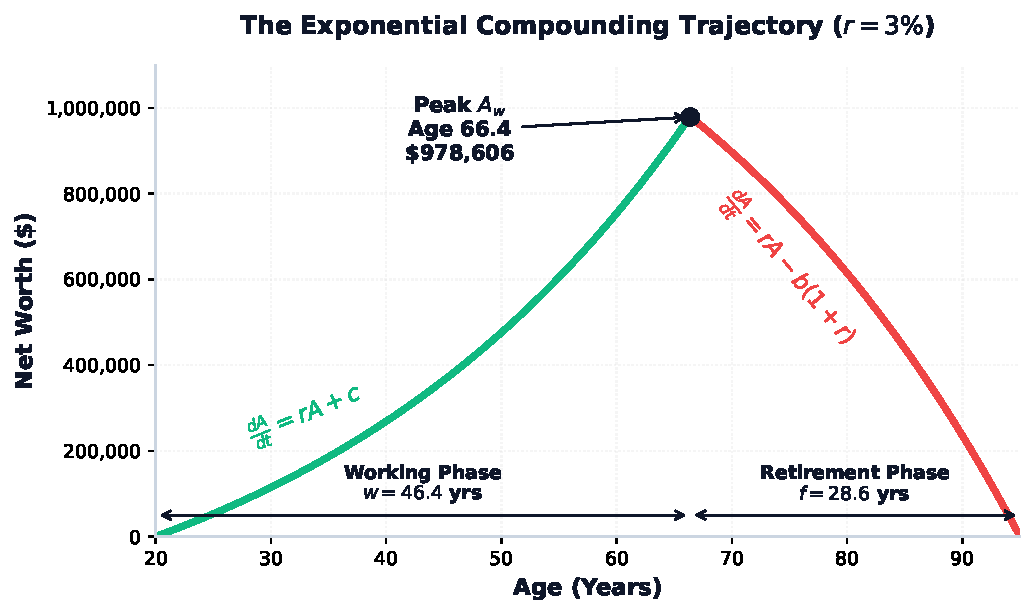
\includegraphics[width=12cm, height=6cm]{exponential_plot.pdf}
    \caption{The exponential compounding lifecyle curves where $r>0\%$. The \textcolor{mpgreen}{accumulation phase} curves upward via geometric expansion and transitions to an accelerated annuity-due \textcolor{mpred}{depletion} phase.}
    \label{fig:exponential_plot}
    \end{figure}

    % =========================================================================
    % SECTION: PLOT 3 (COMPARISON TRAJECTORY)
    % =========================================================================
    \begin{figure}[H]
    \centering
    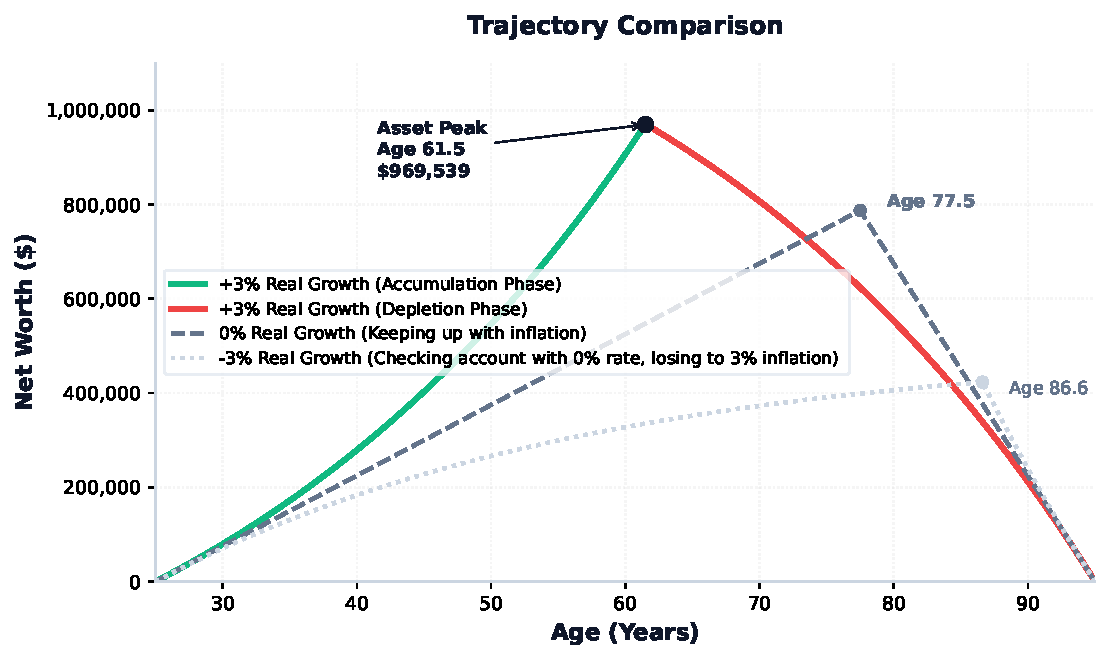
\includegraphics[width=12cm, height=6cm]{comparison_plot.pdf}
    \caption{The exponential compounding curve compared to both assets just keeping with inflation and assets losing to inflation. }
    \label{fig:exponential_plot}
    \end{figure}
    \end{document}